\label{sec:tempered-noise}
\subsection{A normalized prior with controlled moments}

    REV-11 establishes that the original lognormal noise-SD priors give
    infinite response-scale predictive means. We now construct a separate
    exploratory prior family that controls the required moments while
    preserving unbounded positive support. Integrability of quantities of
    interest is part of specifying a Bayesian inverse problem
    \citep{stuart2010inverse}; the following bound is derived here for these
    observation models. The original priors, saved fits, and prospective
    draft are retained as separate records.

    For each noise SD \(v\in\{a,b\}\), put \(z_v=\log v\) and define
    \[
        p_\eta(z_v)
        =\frac{1}{Z_\eta}
            \frac{\exp[-(z_v-\mu_\eta)^2/2]}{\sqrt{2\pi}}
            \exp[-\eta e^{2z_v}],\qquad \eta>0,
    \]
    with
    \[
        Z_\eta
        =\mathbb E_{Z\sim\mathcal N(\mu_\eta,1)}
            [\exp(-\eta e^{2Z})].
    \]
    The SD density includes the usual \(1/v\) transformation factor; the
    posterior is sampled in \(z_v\), where no extra Jacobian is needed.
    Both latent and measurement SDs receive this prior independently.
    Controlling only measurement noise would leave the latent amplitude
    without the exponential-square integrability used below.

    The Gaussian kernel location \(\mu_\eta\) is calibrated so that
    \(\Pr_\eta(v\le0.03)=1/2\). Its kernel scale remains one. Neither
    location nor scale is a moment of the non-Gaussian tempered log-SD
    prior. One-dimensional quadrature computes the normalizer and CDF;
    a scalar root solve matches the median. Independent integration in the
    SD coordinate verifies normalization and the change of variables.
    Matching medians does not match the whole prior: the upper quantiles
    and central shape change, as reported in Table~\ref{tab:tempered-priors}.
    These are declared analyst choices on dimensionless log-response SDs,
    not elicited experimental information or estimates of physical bounds.

\subsection{Global posterior moment bound}

    Let \(N\) be the number of training scalar responses and \(D\) the
    observed data. Conditional on the latent process, the measurement
    likelihood obeys
    \[
        L(D\mid\theta,U)\le C_D b^{-N},
    \]
    where \(C_D\) is finite for the positive observed responses. For a new
    observation and any \(q\ge0\), the logistic median obeys
    \(m_\theta(s_*)\le K\), and the stationary Gaussian discrepancy and new
    measurement error give
    \[
        \mathbb E[Y_*^q\mid\theta]
        =m_\theta(s_*)^q
            \exp\!\left[\frac{q^2}{2}(a^2+b^2)\right].
    \]
    Let \(G_\eta\) denote the product of the Gaussian kernel priors before
    the noise penalties, and let \(Z_D>0\) be the data normalizer under the
    new prior. Using nonnegative integrands and the likelihood bound before
    integrating the latent process gives
    \begin{align*}
        \mathbb E_\eta[Y_*^q\mid D]
        &\le\frac{C_D}{Z_D Z_\eta^2}
            \mathbb E_{G_\eta}\!\left[
                K^q b^{-N}
                e^{(q^2/2-\eta)(a^2+b^2)}
            \right]\\
        &\le\frac{C_D}{Z_D Z_\eta^2}
            \mathbb E_{G_\eta}[K^q b^{-N}]<\infty,
            \qquad \eta\ge q^2/2.
    \end{align*}
    The last expectation is finite because the logistic capacity has all
    positive moments under its Gaussian log-coordinate priors and the
    lognormal measurement SD has all negative power moments. The same
    likelihood bound makes \(Z_D\) finite and positive. This argument applies
    to both temporal kernels and both sharing assumptions. It avoids any
    unproved uniform bound on conditional Gaussian interpolation weights.

    The boundary is included. Conversely, when \(q^2/2>\eta\), the
    large-\(b\) first-moment argument from the preceding section becomes
    a \(q\)-moment integrand with log asymptotic
    \[
        (q^2/2-\eta)e^{2z_b}
        -\frac{(z_b-\mu_\eta)^2}{2}-Nz_b+O(1),
    \]
    which diverges on a positive-volume compact set of the other parameters.
    Thus positive response moments exist exactly through order
    \(\sqrt{2\eta}\), inclusive. The main choice \(\eta=2\) gives a finite
    mean and variance; the fixed sensitivity choice \(\eta=8\) additionally
    gives a finite fourth moment. Neither choice makes every response moment
    finite. The exponential-square prior moment identity
    \[
        \mathbb E_\eta[e^{t v^2}]
        =\frac{Z_{\eta-t}(\mu_\eta)}{Z_\eta(\mu_\eta)},
        \qquad t\le\eta,
    \]
    supplies an independent numerical check, including \(t=\eta\), where
    \(Z_0=1\). The location in the numerator stays \(\mu_\eta\); it is not
    recalibrated for \(\eta-t\).

\subsection{Fixed comparison and computational checks}

    All four discrepancy models are refitted at cutoffs 108, 120, 132, 144,
    156, and 168 for \(\eta=2\), and at 108, 120, 132, and 168 for
    \(\eta=8\): 40 cases. Tail strengths are fixed by the moment requirements,
    not selected by coverage. Other parameter priors and likelihoods are
    unchanged. No historical posterior archive is reused under the new prior.
    Four chains retain the existing warmup-only adaptation and numerical
    acceptance gates; lengths extend only when computation checks fail.

    In addition to coordinates and physical parameters, diagnostics monitor
    the conditional response-mean integrands at the first and last forecast
    times. These checks use every eighth retained draw, with raw ESS and an
    estimated MCSE alongside rank/folded split \(\widehat R\), bulk ESS,
    and tail ESS. Raw mean ESS must also be at least 400. Finite second
    response moments imply a finite variance of the conditional-mean
    integrand by Jensen's inequality. A Markov-chain central limit theorem
    still needs mixing assumptions; existence of the moment alone does not
    prove it. Reported MCSEs are estimates, not rigorous tail-error bounds.

    The main-prior one-step comparison retains 15 distinct scalar targets
    across the five origins. The multi-time comparison retains 36 overlapping
    entries across the first three origins. These are the same previously
    analyzed trial trajectories, not new independent experiments. Full-data
    cases report parameter summaries and a hypothetical next-time forecast
    without observed target scores. Noise-prior normalizers, sources, seeds,
    package versions, numerical settings, and data hashes are recorded per case.

% Generated by scripts/build_tempered_tables.py; do not edit manually.
\begin{table}[htbp]
\centering
\caption{Normalized noise-SD priors: median matched to 0.03. Gaussian kernel locations are not means of the tempered log-SD distribution.}
\label{tab:tempered-priors}
\begingroup\small\setlength{\tabcolsep}{4pt}
\begin{tabular}{rrrrrr}
\toprule
$\eta$ & Kernel location & $\log Z_\eta$ & SD 5th & SD median & SD 95th \\
\midrule
0 & -3.50656 & 0.00000 & 0.00579 & 0.03000 & 0.15541 \\
2 & -3.49260 & -0.01181 & 0.00584 & 0.03000 & 0.14834 \\
8 & -3.45864 & -0.04143 & 0.00596 & 0.03000 & 0.13590 \\
\bottomrule
\end{tabular}
\endgroup
\end{table}
\begin{table}[htbp]
\centering
\caption{Tempered-prior multi-time holdouts: 36 overlapping entries per row. Lower IS and negative log predictive density are preferable.}
\label{tab:tempered-rollout}
\begingroup\small\setlength{\tabcolsep}{4pt}
\begin{tabular}{lrrrrrr}
\toprule
Model & $\eta$ & Cov. & Width & IS & Marg. NLL & Joint NLL \\
\midrule
Independent Mat\'ern & 2 & 0.8056 & 5.857 & 10.149 & 2.403 & 2.189 \\
Independent OU & 2 & 0.8056 & 5.878 & 10.092 & 2.398 & 2.188 \\
Shared Mat\'ern & 2 & 0.9444 & 8.827 & 9.514 & 2.310 & 2.300 \\
Shared OU & 2 & 0.9722 & 9.161 & 9.449 & 2.272 & 2.280 \\
Independent Mat\'ern & 8 & 0.8056 & 5.852 & 10.209 & 2.412 & 2.196 \\
Independent OU & 8 & 0.8056 & 5.875 & 10.122 & 2.400 & 2.191 \\
Shared Mat\'ern & 8 & 0.9444 & 8.870 & 9.401 & 2.310 & 2.297 \\
Shared OU & 8 & 0.9722 & 9.094 & 9.360 & 2.271 & 2.280 \\
\bottomrule
\end{tabular}
\endgroup
\end{table}
\begin{table}[htbp]
\centering
\caption{Main prior ($\eta=2$), one-step forecasts: 15 distinct scalar targets from the same three trial series. Both mean and median point errors are shown.}
\label{tab:tempered-one-step}
\begingroup\small\setlength{\tabcolsep}{4pt}
\begin{tabular}{lrrrrrr}
\toprule
Model & Cov. & RMSE (mean) & RMSE (med.) & IS & Marg. NLL & Joint NLL \\
\midrule
Independent OU & 0.8667 & 1.926 & 1.945 & 8.221 & 2.096 & 2.059 \\
Shared OU & 0.9333 & 1.623 & 1.654 & 7.454 & 1.992 & 2.118 \\
Independent Mat\'ern & 0.8667 & 1.932 & 1.951 & 8.249 & 2.102 & 2.064 \\
Shared Mat\'ern & 0.9333 & 1.722 & 1.756 & 7.829 & 2.034 & 2.133 \\
\bottomrule
\end{tabular}
\endgroup
\end{table}
\begin{table}[htbp]
\centering
\caption{Full-data capacity posterior for the main tempered prior ($\eta=2$). Intervals describe parameters, not new noisy responses.}
\label{tab:tempered-capacity}
\begingroup\small\setlength{\tabcolsep}{4pt}
\begin{tabular}{lrrr}
\toprule
Model & Median & 5th percentile & 95th percentile \\
\midrule
Independent OU & 48.037 & 47.193 & 49.079 \\
Shared OU & 48.357 & 45.704 & 52.306 \\
Independent Mat\'ern & 48.013 & 47.217 & 48.983 \\
Shared Mat\'ern & 48.175 & 46.303 & 51.234 \\
\bottomrule
\end{tabular}
\endgroup
\end{table}


\subsection{Results and interpretation}

    Under the main tempered prior, independent OU multi-time coverage is
    0.8056, with interval score 10.092
    and finite-mean forecast RMSE 2.406.
    Shared OU coverage is 0.9722, with interval score
    9.449 and RMSE 2.191.
    Mean observed-minus-mean-forecast bias remains
    1.642 and 1.370, respectively.
    These results address the moment pathology while retaining the late
    underprediction as a separate model-adequacy issue.

    The historical finite-subset independent and shared OU interval scores
    were 10.164 and
    9.371; their coverages were
    0.8056 and
    0.9722. Those earlier mean-based quantities
    remain finite-subset diagnostics. The new predictive means have a
    mathematically finite target under the new priors. This does not make
    small differences in retrospective scores statistically decisive.

    At the 15 distinct one-step targets, independent and shared OU coverages
    are 0.8667 and
    0.9333. Their mean-forecast RMSE values are
    1.926 and
    1.623; median-forecast RMSE values are
    1.945 and
    1.654.
    Joint density scores retain the modeled dependence between trial
    responses. Table~\ref{tab:tempered-one-step} reports all four models;
    Table~\ref{tab:tempered-rollout} retains both prespecified tail strengths.

    All 40 cases meet the computation gates. The largest monitored
    $\widehat R$ is 1.0059, minimum bulk ESS
    929, and minimum tail ESS
    423. The minimum raw ESS for monitored
    conditional-response-mean observables is
    948; their largest estimated MCSE
    is 0.0717 response units. Those
    functional diagnostics use every eighth retained draw. New fits retain
    36000 to 108000
    draws per chain after 6000 warmup iterations. They support a finite-run
    computation check, not a proof of convergence or predictive calibration.

    For the two main-prior OU models at cutoff 132, posterior integration
    using 6000, 12000, and 24000 components shifts means by at most
    0.014 response units and interval
    endpoints by at most 0.015
    relative to the 6000-component result. These are numerical sensitivity
    checks, distinct from the analytic moment bound.

    No discrepancy model or tail strength is promoted to the mechanistic
    reference. Prior medians are matched, but prior shapes and upper
    quantiles change. Only two fixed tail strengths were tested here;
    the earlier half/double noise-median sensitivity is not a sensitivity
    analysis of this new family. The proposed prospective protocol retains
    its earlier priors and median point forecast until explicitly amended.
    Unconfirmed physical units, experimental dependence, and unavailable
    independent trajectories remain unresolved. A finite predictive mean
    resolves REV-11's mathematical concern for this new family, while
    REV-07's predictive adequacy and REV-10's experimental validation remain open.

\begin{figure}[htbp]
    \centering
    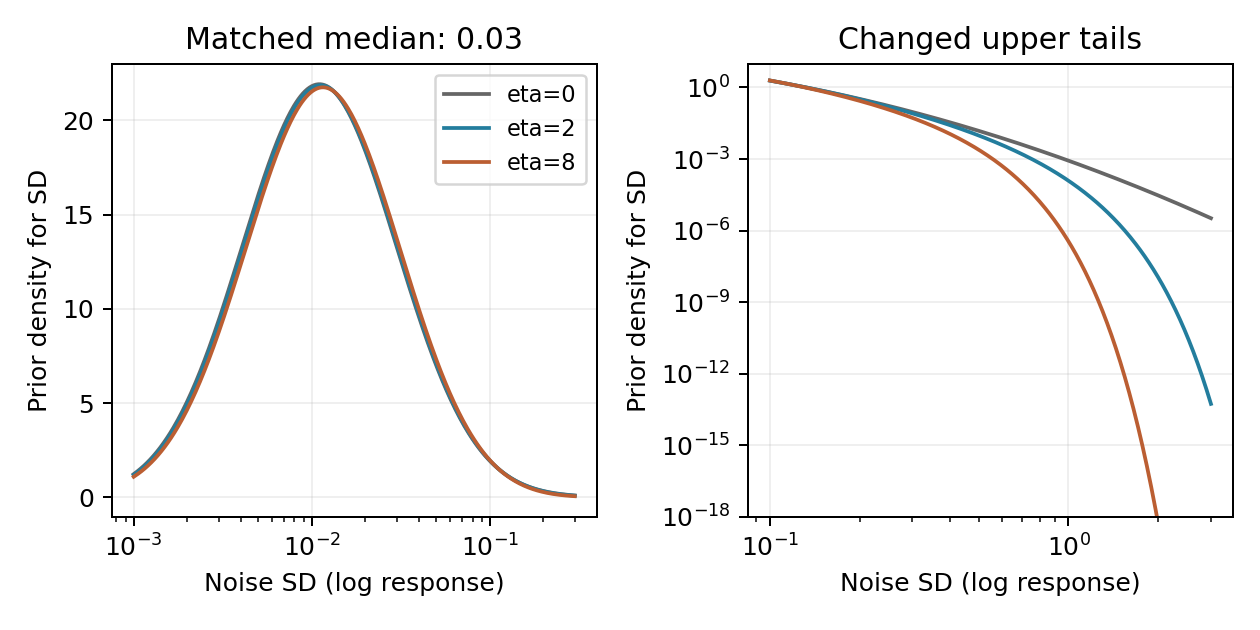
\includegraphics[width=\textwidth]{../results/tempered/noise_prior_comparison.png}
    \caption{Noise-SD prior densities with matched median 0.03. The stronger
    upper-tail penalties change the 95th percentiles and tail integrability;
    they impose no finite upper SD bound. Both latent and measurement SDs
    receive the same separate prior.}
    \label{fig:tempered-priors}
\end{figure}
\begin{figure}[htbp]
    \centering
    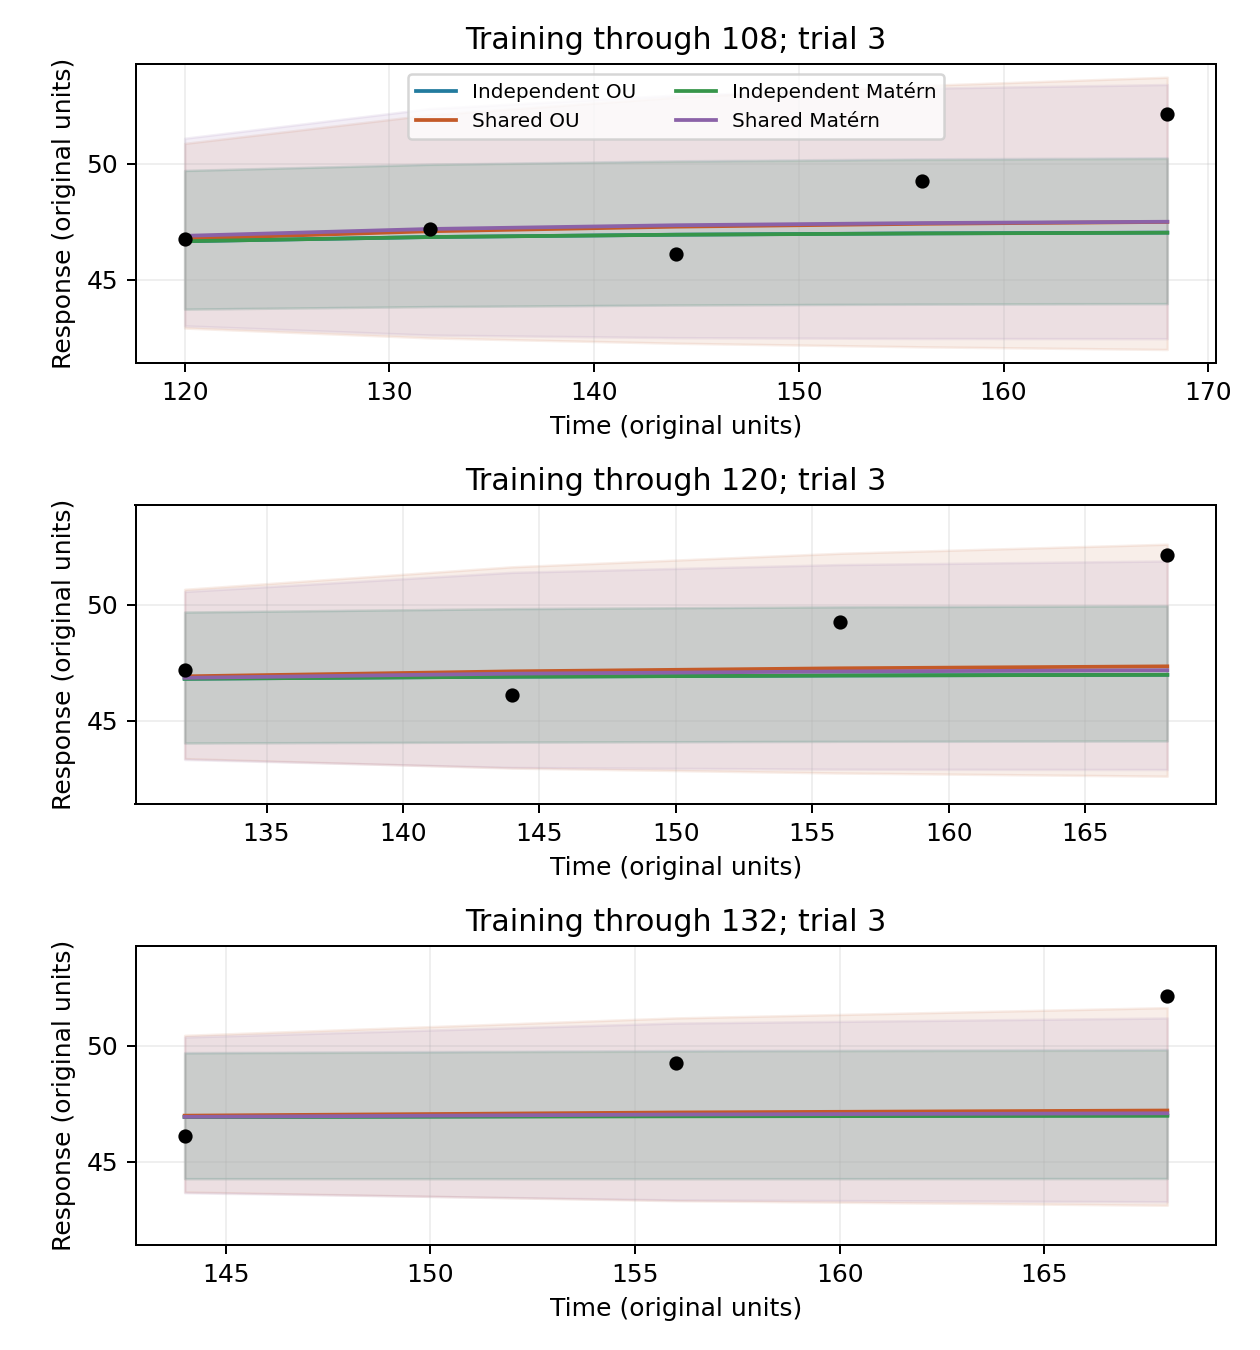
\includegraphics[width=\textwidth]{../results/tempered/forecast_comparison.png}
    \caption{Main tempered prior: trial 3 predictive means and central
    90 percent observation intervals. Black points are held-out responses.
    All reported metrics use the three trial series. These means estimate
    finite response expectations under the new model.}
    \label{fig:tempered-forecast}
\end{figure}

